\documentclass[titlepage]{article}

\usepackage[english]{babel}
\usepackage[a4paper, left=2cm, right=2cm, top=2cm, bottom=2cm]{geometry}
\usepackage{amsmath}
\usepackage{graphicx}
\usepackage{placeins}
\usepackage[table]{xcolor}
\usepackage[colorlinks=true, allcolors=blue]{hyperref}
\usepackage[acronym]{glossaries}
\usepackage[parfill]{parskip}
\usepackage{listings}

\bibliographystyle{IEEEtran}
\graphicspath{{figures/}}
\makenoidxglossaries

\newacronym{ram}{RAM}{Random Access Memory}
\newacronym{gpu}{GPU}{Graphics Processing Unit}
\newacronym{cpu}{CPU}{Central Processing Unit}
\newacronym{api}{API}{Application Program Interface}
\newacronym{opengl}{OpenGL}{Open Graphics Library}
\newacronym{webgl}{WebGL}{Web Graphics Library}
\newacronym{dda}{DDA}{Digital Differential Analysis}
\newacronym{lod}{LOD}{Level of Detail}
\newacronym{svo}{SVO}{Sparse Voxel Octree}
\newacronym{fov}{FOV}{Field of View}
\newacronym{ecs}{ECS}{Entity Component System}
\newacronym{jit}{JIT}{Just in Time}
\newacronym{dry}{DRY}{Don't Repeat Yourself}
\newacronym{fps}{FPS}{Frames per Second}
\newacronym{qut}{QUT}{Queensland University of Technoloogy}

\begin{document}

\begin{titlepage}
  \begin{center}
    \vspace*{7cm}

    \Huge
    \textbf{Creating a Voxel Rendering Engine}

    \vspace{0.5cm}

    \Large
    EGH400-2 Project Delivery - Semester 1, 2023

    \vspace{0.25cm}

    \large
    Supervised by Professor Clinton Fookes

    \vspace{0.5cm}

    \Large
    \textbf{Alex McDermott (N10494367)}

    \vfill

    \Large
    The Queensland University of Technology\\
    \today
  \end{center}
\end{titlepage}


\begin{abstract}
  The aim of this thesis project was to assess the feasibility of a real time voxel rendering engine in the browser. This was done with the intention of potentially making this application available for medical use, allowing exploration of medical scans in a more intuitive manner from any internet connected computer. Assessing the relevant literature and research already done in this space, this paper explores voxel data generation, storage and rendering, touching on algorithms such as \gls{dda}. Despite using a rudimentary fixed step size ray marching algorithm for its own implementation, the performance demonstrated here is still well above the 60 \gls{fps} real time rendering target. Achieving a locked 120 \gls{fps} on the test hardware, this implementation is well suited for the web and is a promising proof of concept for future work. This paper also explores the potential for future improvements and optimisations, such as \gls{dda}, WebGPU, and more advanced shading.
\end{abstract}

\tableofcontents
\listoffigures
\printnoidxglossary[type=\acronymtype]
\newpage

\section{Introduction}

The primary goal of this research project was to create a voxel rendering engine; with a secondary objective of utilising flexible technology to allow for the engine to be used across a variety of platforms, mainly the web. Firstly, what is a voxel, let alone a voxel rendering engine. A voxel is essentially a 3D pixel, and is a common way of representing volumetric data such as clouds, medical scans, and destructible terrain as seen in games, tv shows and movies. As opposed to traditional rendering, that utilises triangles to approximate surface geometry, a voxel render uses a fixed grid of evenly spaced voxels where each voxel stores information about the object they are approximating in that particular point in space. Primarily this is whether the cell is filled (transparent or opaque) or not. This allows for a more intuitive representation of reality as these voxels mimic particles and allow for easy manipulation of objects as we've come to expect in everyday life. There are more advantages to voxels as well as drawbacks that will be discussed in this report, along with techniques that can be used to mitigate them. This thesis aims to assess the feasibility of this sort of application in the browser with potential for use in interactive medical visualisations. In summation, the core goals of this thesis are outlined below.

\begin{itemize}
  \item Generate a voxel representation of an object.
  \item Implement an algorithm to directly render this data structure without the need for intermediary processing such as meshing into triangles.
  \item Assess the implementation and its feasibility for web platforms.
  \item Identify future improvements and optimisations given performance budget.
\end{itemize}

\section{Literature Review}

Before delving into the existing research done in this field, I'd like to provide some context for this project. Due to unforeseen reasons in the first half of this project, my original thesis plans with Airbus fell through as they where unable to find a suitable supervisor to manage the project. Hence, in Week 10, I switched to this project, having little background knowledge as my Literature Review was done with regards to the original topic Airbus proposed. As such, development in this second thesis unit has been slow as a significant amount of time was spent researching and understanding existing work which would ideal have been completed in the first half of the project. Because of this, the scope of the final implementation is quite limited but I believe the assessment was still highly beneficial, leaving room for many future improvements and expansions on current work.

\subsection{Voxel Storage}

\subsubsection{Data Structure}
The first and most prevalent technique is to utilise a data structure called a \gls{svo}. An \gls{svo} operates on the same principle as a quadtree, such as those used to minimise checks against distant objects in 2D collision detection. It's a 3D tree structure that iteratively subdivides itself as necessary down to a given depth depending on the resolution needed. This technique is documented well in literature, but is particularly well explained in this paper on ``Efficient sparse voxel octrees'' \cite{octree} where their explanation is accompanied by this visualisation showing how tree depth level allows approximation of more precise geometry.

\begin{figure}[htp]
  \centering
  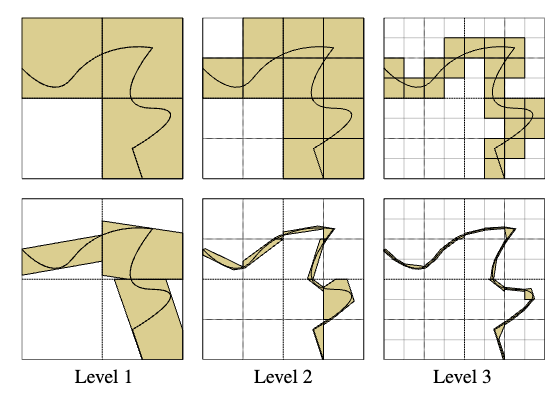
\includegraphics[width=0.7\textwidth]{octree.png}
  \caption{How octree depth affects volume \gls{lod}.}
\end{figure}
\FloatBarrier

To provide an example of how this is useful, lets say we have a scene that has some ground, a house, some empty space above it and them some clouds in the sky; all represented in voxels. Representing this scene in an octree we surround it by a single cube bounding box (proxy geometry), this cube is then split into 8 smaller cubes because there is lots of geometry that needs to be represented, these smaller cubes are called octants. This idea of proxy geometry is inspired by the voxel game Teardown \cite{proxy} where they use a similar technique to compose scenes of multiple separate voxel objects. The octans created by subdividing this proxy geometry are essentially smaller voxel volumes and they keep repeating this splitting process until a set tree depth is reached. The benefit of this is that, when an octant has no voxels it in, it has no reason to keep subdividing. Considering out example scene allows the empty sky to essentially be represented by one large voxel that can be quickly jumped over when traversing this structure at render time. More importantly, if we assume our sky took up $\frac{1}{3}$ of our scene this equates to a around a 33\% reduction in voxel memory footprint as it can now be stored as a single byte as all the voxels in that region are of a single empty type. This reduction by itself is already a significant saving, and when applied to a whole scene this effect is compounded over all the empty space such as inside the house, around the clouds, and possible caves underground. These savings add up and drastically reduce \gls{gpu} memory footprint and bandwidth usage.

\subsubsection{Compression and Voxel Representation}
As stated previously, voxel data is often stored in an evenly spaced 3D grid of voxels. In its simplest form, this can mean each voxel only needs to store a single bit, either 1 or 0 depending on whether the voxel is filled or not. Although this is very rarely the case in actual implementations as things such as different materials, densities, normal information, colours, and more, are likely also stored in the voxel. Lets instead assume that each voxel is represented by a byte or 8 bits. This gives us the flexibility to either store an index that could possibly map too 255 different predefined materials or if more control is need, bit packing could be employed with a custom encoding format to store this information in the byte directly. To provide a basic example illustrating this, if we assume a hypothetical voxel volume size of $512^3$, with each voxel being 1 byte each, this already consumes around 135 MB of memory. This may not seem like a lot, seeing as its common for modern computers to have upwards of 8 GB of memory, although since voxel rendering is primarily a \gls{gpu} process, this is memory will be stored in video \gls{ram} which is much less prevalent and often tightly budgeted. This high memory footprint is one of the primary drawbacks of voxel usage. Fortunately, there are many techniques that can be used to reduce the memory footprint of voxel data. The paper ``Geometry and Attribute Compression for Voxel Scenes'' \cite{compression} explores this pallet based compression scheme and aims to decouple voxel geometry from attribute data such as color and normal information. In their highly detailed test scenes, they show reduced ``memory usage from 4.49 times (for the citadel) up to 11.5 times (for San Miguel)'' using this method.

Another common technique that can be used to reduced the memory footprint of storing voxel volumes is run length encoding. Run length encoding is a lossless form of data compression that simply counts how many times the same value occurs in a sequence and stores that value along with the count. This is useful in the context of voxels as it is common for many of the same type to appear next to each other such as dirt on the ground, or air blocks in the sky. Lets assume we are looking at a leaf octant of the \gls{svo} that is $16^3$ voxels in size. If we assume that this octant is filled with air, we can store this entire octant in a single byte as we know that all the voxels in this octant are of the same type. This is a very simple example and in reality, the savings will be much less when applied over a whole scene especially with lots of variation but it still shows the potential for compression in voxel data.

\subsubsection*{Streaming}
Streaming is another technique that can be used to reduce the memory footprint of voxel data. Streaming is the process of only loading the data that is needed at a given time. This is why you sometimes get a loading screen when going through doors in open world games, it gives the game time to load in all the models, textures and data related to that section of the game. In voxel applications, steaming is often implemented by ``chunking'' the environment into smaller, more manageable sections. Many have most likely seen this idea implemented in Minecraft \cite{minecraft} where sometimes artefacts can be seen where chunks are yet to be generate or load in, leaving cube sized holes in the map. Chunking also works well with the octree solution we previously talked about, as only specific nodes of the octree need to be loaded into memory depending on where the observer is in the scene. Voxel steaming can be implemented to only load data into the \gls{gpu} that is actual visible to the observer, allowing large savings in memory footprint as the need to store information on data outside the players \gls{fov} (such as behind them) is no longer needed. To provide an example, a typical \gls{fov} in games is around 60 degrees, lets assume a worst case scenario, where want to load in 180 degrees worth of voxels so the games doesn't lag while steaming in new data when rotating. Assuming the player is centred in the voxel space, this automatically discounts 50\% of the scene that doesn't need to be loaded into \gls{gpu} memory and thus a large saving in memory footprint. This idea can be seen documented in the paper ``Gigavoxels: Ray-guided streaming for efficient and detailed voxel rendering'' \cite{streaming} where they state: ``for a given point of view, not the entire volume needs to be in memory. By organizing the data in a spatial sub-division structure, empty parts can be let un-subdivided and distant parts can be replaced by lower mipmap levels, leading to \dots less \gls{gpu} memory requirements''. Here, the validity of only loading needed parts of the voxel volume is solidified. They also suggest another good optimisation; taking advantage of the iteratively increasing detail at deeper levels of the \gls{svo} structure, to reduce the number of ray traces, distance octree volumes can be limited in how far they traverse down the tree. This leaves more processing power for closer objects which take up a proportionally larger area on the screen. They illustrate this idea well in the following figure included in their paper.

\begin{figure}[htp]
  \centering
  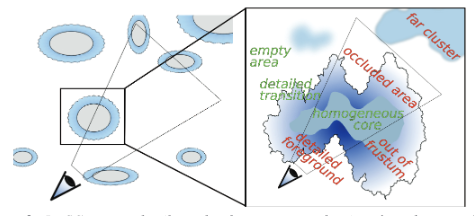
\includegraphics[width=0.7\textwidth]{frustum.png}
  \caption{Visualisation of the camera frustum culling and dynamic \gls{lod}.}
\end{figure}
\FloatBarrier

These are the three primary and most effective techniques used to reduce the memory footprint of voxel volumes. As stated, this is important as the less space a voxel takes up, the more of them we can store, opening up opportunities to represent more detailed and complex scenes. Having a small voxel footprint is also beneficial when it comes to render time as well, seeing as the voxel data has to be transferred between the \gls{cpu} and \gls{gpu} potentially every frame if updates have occurred. These transfers are expensive and a notorious bottleneck in graphics programming. This is another reason why it is important to keep the voxel footprint as small as possible, to reduce the amount of data that needs to be transferred between the \gls{cpu} and \gls{gpu}.

\subsection{Voxel Rendering}

\subsubsection{Graphics APIs}
Now that we have a basic understanding of how voxel data is stored and streamed efficiently, we can look further into how this data is displayed. As stated, voxel rendering is primarily a \gls{gpu} process, and as such, we will require a means to communicate this data to the \gls{gpu} device. This is often done using one of the four core main graphics \glspl{api} being Metal, Vulkan, \gls{opengl}, or DirectX. These libraries are responsible for telling the \gls{gpu} what to draw, where to draw it, and how to do it. As such they are notoriously low level and require a large amount of boilerplate code to get set up. Fortunately in the browser, we have two alternatives \gls{webgl} and WebGPU, they are essentially wrappers around these low level graphics \glspl{api} that are designed to be more accessible and provide the functionality needed in the browser. The first of which, \gls{webgl}, was first released in 2012 and based on \gls{opengl}. \gls{webgl} is very mature, meaning there is plenty of documentation and examples available online. Although being more than a decade old, graphics hardware and rendering technology has come a long way in this time, and as such \gls{webgl} is not as efficient as modern graphics libraries such as Vulkan. WebGPU on the other hand is actually based on Vulkan and is designed to be an extensible replacement to \gls{webgl} that is more modern and efficient. Because of this, and due to the high performance nature of the application being built as part of this thesis, WebGPU was initially chosen as the target for this project. Although after difficulties finding learning resources, limited documentation and changing specifications as the \gls{api} is still being finalized, it was deemed to not be production ready yet. As such, the project was switched to use \gls{webgl} as it is more mature and has a larger community and support base. Although this switch was a setback in terms of the project timeline, it was greatly beneficial in terms of utilisation of existing resources. In addition to this, instead of utilizing the \gls{webgl} \gls{api} directly, a third party library called ThreeJS was used which provides yet another abstraction on top of \gls{webgl} to make it even more accessible. This was done in the interest of further reducing boilerplate code, as well as looking to future proof the project since the core developers of ThreeJS have already stated that they will be porting the library to WebGPU once it is production ready. This allows the program to utilize the stability and knowledge of the \gls{webgl} ecosystem while still being able to easily port to WebGPU and reap its performance benefits once it is production ready.

\subsubsection{Rendering Approach}
Now that a means of communication has ben established with the \gls{gpu}, a technique is needed to actually render voxels to the screen. As previously stated, the goal of this voxel renderer is to directly draw the voxel data as opposed to meshing the voxel geometry into triangles and rending that; which is a common approach used in games such as Minecraft. The reason this approach is so prevalent is because of how \gls{gpu} architecture has evolved over time. As triangles are so versatile, and essentially the foundation for all 3D representations of objects seen in movies, tv shows and video games, \gls{gpu} hardware as evolved to accommodate this. Leading to decades of \gls{gpu} optimisations and design choices made with triangle rendering in mind as it is by far the dominate way to represent geometry. This makes meshing voxels into triangles using algorithms such as marching cubes, such a popular approach as it leverages these optimisations and additional hardware acceleration. This is not to say rendering voxels isn't possible or impractical, just that it is not as common and requires a different approach. This approach is called ray tracing, specifically, ray marching. It works by casting a ray from our camera, into the scene and ``marching'' along that ray, incrementally extending it and testing if a voxel has been hit. This is a vast simplification of a complex topic who's implementation will be explored later in this paper. A drawback of this approach is that ray casting can be quite expensive, especially when multiple rays are cast per pixel, per frame, 60 times per second. At common resolutions such as 1080p that could easily require north of 100 million rays cast per second assuming two samples per pixel. This might sound like overkill or an unrealistic scenario but casting multiple rays per pixel is extremely common in ray tracing applications as it is often used to average sample values and decrease noise, or needed to calculate visual effects such as shadows, reflections, and refractions.

\subsubsection{The DDA Algorithm}
Having realized the performance pitfalls of our selected rendering approach, it is important that the algorithm we implement be as efficient as possible if this approach is to be feasible within the browser. Knowing that we need to march a ray through our voxel space, a naive approach is to take steps of fixed size along the ray. This is problematic for two reasons. Firstly, when taking fixed step sizes over an axis-aligned volume of cubes at an arbitrary angle, it is possible to skip over voxel checks along the ray's path if a step happens to skip over a voxel corner (being less wide than a voxel's diagonal). This can lead to artifacts of voxel edges. Secondly, this approach is also flawed from a performance standpoint as well. Taking fixed step sizes is inefficient when there is potential for optimizations to be made on the account of having a fixed grid of voxels. Fortunately, there is a more performance-oriented approach known as \gls{dda}. \gls{dda} takes advantage of this fixed size grid by ensuring that each step along the ray equates to a movement of exactly one voxel in one and only one of the cardinal directions. This is done by calculating how a steps size of one voxel unit along each cardinal direction will affect the length of the stepped ray; then choosing the axis that results in the smallest ray distance increase, as to not miss voxel checks. This is a vast improvement over the naive approach as the voxel steps size is maximised without skipping checks while the number of voxel check is minimised as each cell is only checked once. A follow up paper \cite{dda} by the authors of ``Efficient sparse voxel octrees'' cited previously visualises these unit size, axis align steps in the figure shown below. This figure shows how the \gls{dda} algorithm is able to take advantage of the fixed grid of voxels by always performing the minimum number of voxel checks at exactly one per ray step.

\begin{figure}[htp]
  \centering
  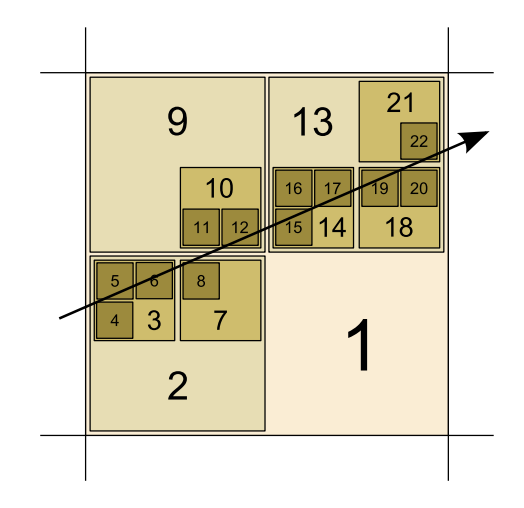
\includegraphics[width=0.7\textwidth]{dda.png}
  \caption{Visualisation of voxels checked when performing the \gls{dda} algorithm}
\end{figure}
\FloatBarrier

\subsubsection{Shading}
Another advantage of the \gls{dda} algorithms stepping approach is the increased accuracy; since the hit position returned will also be the exact position on the boundary of a voxel. Whereas, with a fixed step size approach, the hit position could land anywhere within a voxel's bounds. The benefit of knowing the exact hit position is realized when it comes to handling lighting and shading calculations, as it aids in calculating the volume's normal at the hit position. In 3D graphics, the normal vector at a position is a vector that is perpendicular to the surface at that point. As seen in the paper ``Fast phong shading'' \cite{phong}, the normal direction is foundational in calculating even the most simplistic of lighting models. It allows us to determine how much light is reflected off a surface and is needed for anything more than simple diffuse shading. In the figure seen below, the normal can be seen as the vector perpendicular to the surface at the hit position.

\begin{figure}[htp]
  \centering
  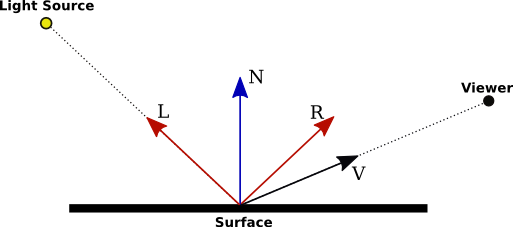
\includegraphics[width=0.7\textwidth]{phong.png}
  \caption{Important vectors involved in Phong shading}
\end{figure}
\FloatBarrier

When shading voxel volumes, there are two approaches that are most commonly taken, depending on the style of render being targeted. If trying to provide a smoother representation of a real-life object, such as a medical scan or cloud volume, normals might be stored directly in the voxel data. This way, no matter the ``face'' of a voxel a particular ray hits, the resulting hit position at each will share the same normal value. This makes the voxel nature of the render less prominent, as there are no shading differences between voxel ``faces''. Alternatively, if one wishes to embrace the voxel art style of the render or if modelling something cube-like already, such as a house, for this case, normals can be calculated in real time. For this voxel rendering engine, the second approach will be targeted for two reasons. Firstly, to highlight the voxel style, and secondly, given the already high memory requirement for voxel data, it is ideal to keep the amount of data stored for each individual voxel to a minimum. As mentioned previously, the \gls{dda} algorithm is very beneficial here, as the required normal is essentially calculated as a by-product of the stepping process. Since the algorithm walks along the voxel boundaries, essentially in the same zigzag nature you see when calculating Manhattan distance, we know which side of the voxel was hit. Combining this with the sign of the ray's direction vector, the normal vector at the hit position can be derived.

\section{Methodology}

As stated at the beginning of the literature review, due to the organisational issues of Airbus and the falling through of our industry partnership, development progress on this thesis was delayed on account of having to redo the literature review. Despite this, a functioning voxel renderer was still created, although sadly many of the optimisations and more advanced techniques mentioned here where not able to be implemented as of yet within the given time frame. This section will outline the technologies that where used, as well as the implementation details of the voxel renderer in its current state.

\subsection{Technology Stack}

\subsubsection{Rust and Bevy}

Upon initial research into the topic of voxel rendering, it was promptly observed that there would be a serious need for highly performant code if this application was going to run in real time in the browser. For this reason, as discussed above, this engine was initially written in Rust using the Bevy \gls{ecs}. This choice was made based on the on the high performance of Rust, its memory safety, and developer appeal as seen in the most recent StackOverflow developer survey where it ranked number one as the most loved language \cite{survey}. Bevy was chosen for similar reasons, it is written in Rust and would provide an abstraction on top of the very performant WebGPU graphics \gls{api}. With both of these technologies being written in Rust, there was also the potential for compilation to Web Assembly which would allow the \gls{cpu} side of the engine to run at native compiled speeds instead of being \gls{jit} compiled by the JavaScript runtime. Despite the incredible performance potential of this technology stack, as mentioned above, due to severely lacking documentation, and the continually evolving specification of WebGPU while it is is being finalised; development was extremely challenging and deemed non production ready as a result of this. Observing the consequences of adopting bleeding edge technology, a step back was taken an the timeline of this project was reassessed in order to reconsider how this implementation could be approached.

\subsubsection{JavaScript, ThreeJS and React Three Fibre}

Given the already short project timeline and after encountering the issues described above; it was decided to switch language to a more stable development platform. The language that was chosen was JavaScript, this was the choice for two primary reasons. Firstly, JavaScript (specifically TypeScript) is the language I am most familiar with myself, which would be beneficial when accounting for the shortened project timeline as minimal time would be spent learning language specific features. Secondly, JavaScript is the native language of the web, making it a natural choice for a browser based application. With JavaScript replacing the language, a replacement would also be needed for the Bevy framework that was previously being used. The replacement that was settled on was ThreeJS, an extremely popular JavaScript library that wraps the \gls{webgl} \gls{api} the same as Bevy wrapped the WebGPU \gls{api}. In the modern web landscape, it is almost always commonplace to use some sort of frontend library when building any sort of web app. For this project I chose NextJS because of its popularity, my personal familiarity with it, as well as its ability to generate static sites which would be beneficial for hosting the final application. In addition to this, I also utilized React Three Fibre as an additional wrapper around ThreeJS allowing me to specify a scene using React components within my NextJS application. This switch to an interpreted language will likely have some kind of performance impact, but given the time saved by not having to learn a new language, and the increased stability of the development environment, it was deemed a worthwhile trade-off. In addition to this, being a predominantly \gls{gpu} bound application, the performance impact of the language choice is likely to be minimal.

\subsection{Voxel Data Generation}

Delving into the working implementation that has been created as part of this project. Before anything can be rendered to the screen, a voxel volume must be created. There are numerous formats that have been created by the community to store voxel data, such as that used by the MagicaVoxel modelling program \cite{magicavoxel}. Although being in the proof of concept stage, it is currently not necessary to implement this functionality and this has been designated as a future improvement if the project is deemed to be feasible for web platforms. Instead, a custom minimalistic approach was taken, as when implementing a new system, less complexity leaves less room for error and allows for easier debugging during the development process. As eluded to above, the format used in this paper simply stores a single number per voxel, whether it is filled or not. The code snippet shown below generates a test scene in the form of a sphere centred around the voxel volumes origin.

\lstinputlisting[firstline=10, lastline=45]{../../app/src/components/VoxelObject.tsx}

Observing the code snippet above, there are a number of notable implementation details that should be discussed. Firstly, is the use of the React useMemo hook; this ensures that this volume generate logic is only run once on the components initial render. This is controlled by the final line of the snippet where the dependency array is has zero elements. This essentially caches the volume and prevents React component updates and hot reloads from regenerating the volume would be inefficient. Secondly is the ``targetResolution'' variable; this is the result of a stylistic decision that I made. I would like the voxels volumes rendered by this engine, to be centred around the middle point of a single voxel to aid in intuitive design, positioning and interaction as opposed to having objects offset to one side. Given an integer value for the targetResolution, performing a bit wise OR with a value of 1 will always produce an odd numbered resolution which is needed to achieve this effect. Related to this, when calculating the spheres radius, a value of resolution minus one is used. This calculates a sphere slightly smaller than the volume as this extra headroom needed to later center the voxels by subtracting half their size in the shader. The third and final notable implementation detail is the use of a Uint8Array for storing the voxel data. This is a typed array that stores 8 bit unsigned integers, in JavaScript this is the most efficient form of array available. Since the number and size of elements are both known, this allows the interpreter to allocate enough memory for the array in advance, as opposed to a traditional array which is dynamically allocated. The use of this array ensues that the voxel data is store in a contiguous block of memory, this is beneficial as it allows for faster operations by utilising the cache more efficiently. Having now declared all the data needed to render this voxel sphere, this information is packed into the uniforms object and transferred to the \gls{gpu} where this information will be rendered.

\subsection{Ray Tracing and Step Size}

Within the shader, we must first receive the uniform values we have passed in as well as the camera position and worldPosition. The worldPosition of our pixel is calculated in the vertex shader and passed in into our fragment shader from there. As seen in the code snippet below along with our received uniforms, the worldPosition is the result of a matrix multiplication with the pixels model space coordinate, multiplied by the model transform.

\lstinputlisting[firstline=12, lastline=1]{../../app/src/shaders/vertex.vs}
\lstinputlisting[firstline=6, lastline=14]{../../app/src/shaders/fragment.fs}

An interesting implementation detail here is that our Uint8Array passed from JavaScript is interpreted by the shader as a sampler3D object. This is due to the fact this data has been parsed as a 3D texture by the GPU, allowing us to index into it with normalised 0 to 1 coordinates to sample the voxel state at a given point. Having now loaded all the required information into \gls{gpu} memory and obtaining references to them in our shader, we can progress to the main logic of the voxel rendered. The algorithm starts as seen below, where a ray is created with its origin at the camera and pointing to the worldPosition of our current pixel (somewhere on the surface of our proxy geometry).

\lstinputlisting[firstline=71, lastline=81]{../../app/src/shaders/fragment.fs}

This small function encapsulates the whole renderer, we can say that if the result of the ray cast is infinity, the pixel will return an all black value represented by the vec4(0.0) where the 4th element indicates an alpha channel of 0 meaning the pixel is transparent. The visualisations produced in the case of a voxel hit will be discussed later in this report during the results section. Flowing on from this, the ray cast function can be seen implemented below. Sadly, as discussed previously in this report, time constrains as well as development difficulties did not allow for implementation of the more efficient \gls{dda} algorithm; hence, this less accurate simpler method uses a fixed step size. Despite this, method is able to produce a visually pleasing result and is a good proof of concept for the project as it represents a worst case scenario. A \gls{dda} implementation would only improve on and deliver more promising performance for a browser implementation and is definitely the number one priority in terms of future implementation. The step size used here is a constant value of 0.01, this was chosen as it is small enough to produce a smooth result but large enough to not be too computationally expensive. This value could be made smaller to increase accuracy at the cost of performance, or larger to increase performance at the cost of accuracy. Although this value cannot be increase in isolation as it has a high interaction with the maxSteps variable. Having a small step size and a low max steps will yield poor results as the ray will not be able to sufficiently explore the voxel space before running out of iterations which can lead only surface or highly extruded pieces of the volume being rendered.

\lstinputlisting[firstline=59, lastline=69]{../../app/src/shaders/fragment.fs}

Having strictly followed the \gls{dry} programming principle and implementing single use composable functions as is best practice; each function is mainly responsible for a single core operation. The rayCast function show above is responsible for the extension of the ray and gradual exploration of the voxel space. Hence we will now look at the lookupVoxel function, which handles bounds checking and extraction of the voxel data from the 3D texture. Seen below, we ensure the index position is in the range zero to one as if we sample outside of this range, the default behaviour of the sampler is to repeat our texture, meaning we will still receive data but it will be incorrect.

\lstinputlisting[firstline=43, lastline=48]{../../app/src/shaders/fragment.fs}

Progressing deeper to the actual index calculation seen in the snippet below, this function covers conversion of the 3D coordinates of a sample position, to the zero to one range required by the voxel data texture lookup. As our proxy geometry is a unit cube centred at the origin, we add 0.5 to all components of the position vector to convert them to the range zero to one. Division via the voxel size (in world space units) then flooring the result converts this float value to zero index integer value. We then add half the voxel size to ensure we sample the center of each voxel to avoid confusion if sampling on a voxel boundary. Finally, we divide by the voxel count to convert the value back to the zero to one range required by the sampler.

\lstinputlisting[frame=single, firstline=35, lastline=41]{../../app/src/shaders/fragment.fs}

\section{Results}

\subsection{Visualisation}

Having now explored the logic and implementation details behind this basic but highly extensible voxel render we are now able to view the results it produces. In the case of a voxel being hit, there is currently two implemented visualisations; the normalised depth, and the voxels position. Firstly the normalised depth can be seen below.

\begin{figure}[htp]
  \centering
  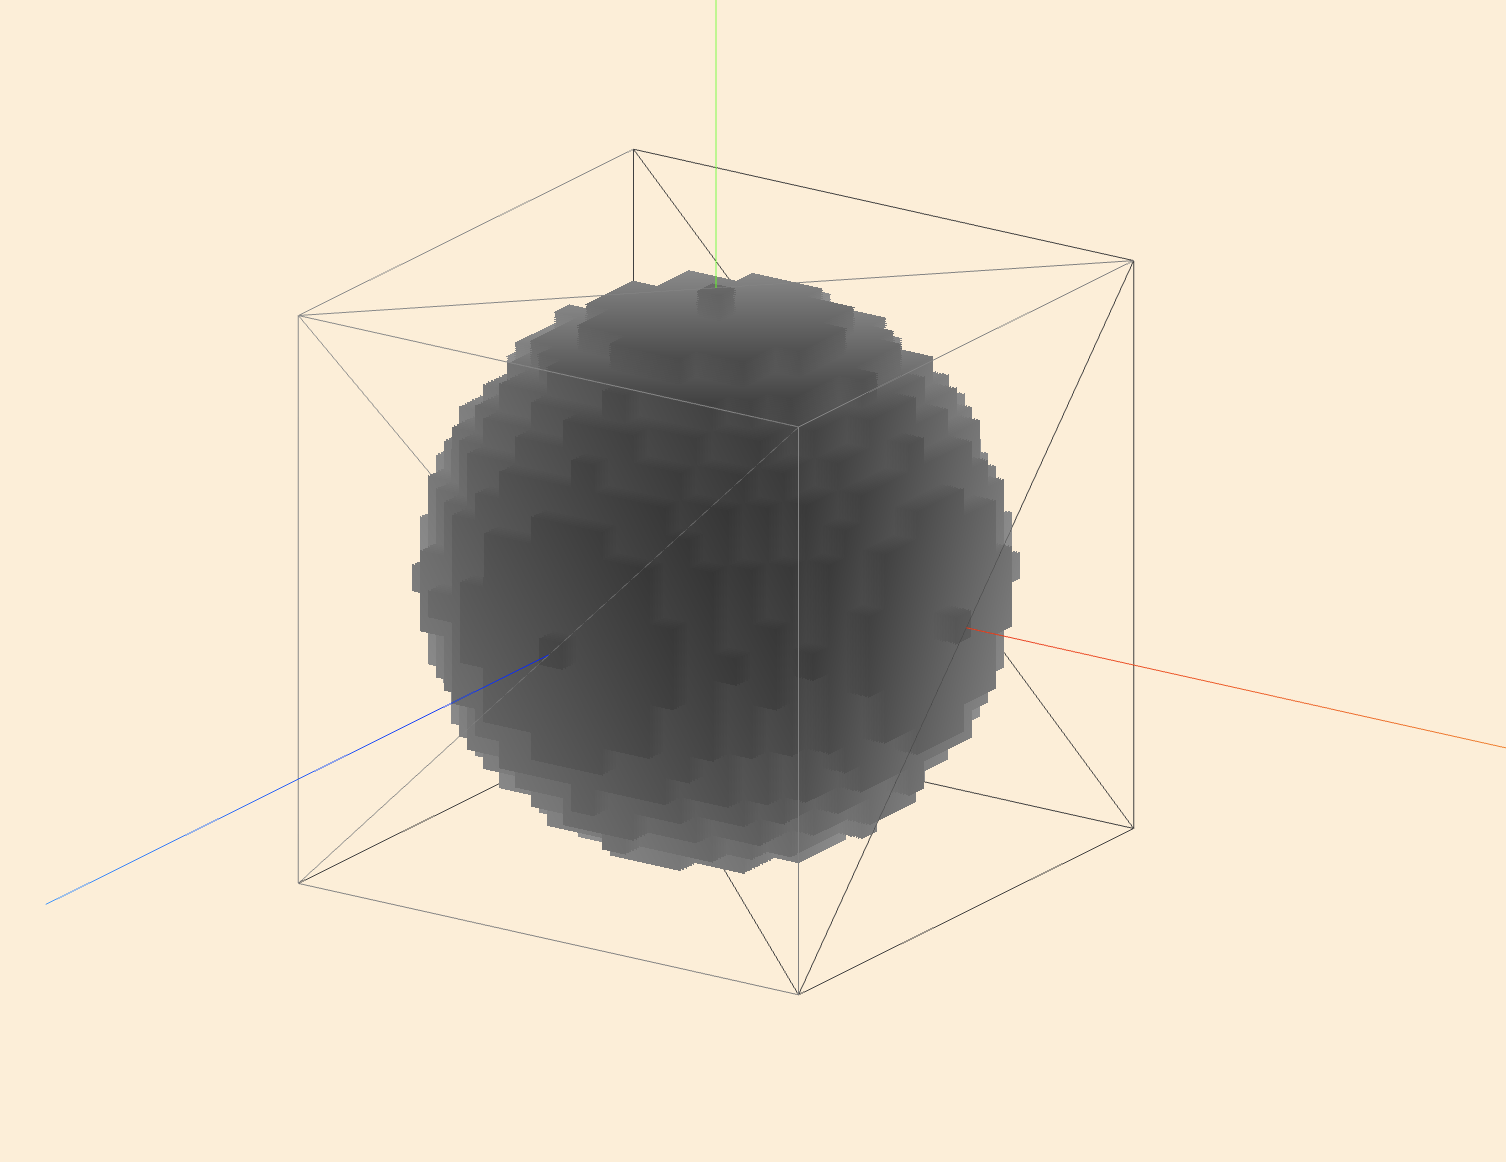
\includegraphics[width=0.7\textwidth]{depth.png}
  \caption{Visualisation of the normalised pixel depth.}
\end{figure}
\FloatBarrier

This depth if said to be normalise as in theory, the ray could potentially progress infinity far into the scene but we are only able to represent colours in the range zero to one. To combat this, before visualisation, the depth value of the hit ray has the distance to the camera subtracted, then is divided by the diagonal width of the voxel volume. This essentially maps the depth value to the range of zero to one, with zero being close to the camera (front of the voxel volume) and one being far away (back of the voxel volume). This logic can be seen implemented in the code snippet below.

\lstinputlisting[firstline=50, lastline=57]{../../app/src/shaders/fragment.fs}

The second visualisation that is currently implemented is the position of the voxel. This render simply colours each pixel by using the voxels position as its colour. This is possible as the proxy geometry is a unit cube centred around the original so all positions are already in the unit range of -0.5 to 0.5 and a simple addition of 0.5 produces the zero to one range of values required for non clamped colouring. An interesting shading effect that arises due to this is that the volume appears slightly shaded as pixels closer to the origin (those making up inset corners) are shaded darker than those closer to the edge of the volume (those on outset corners).

\begin{figure}[htp]
  \centering
  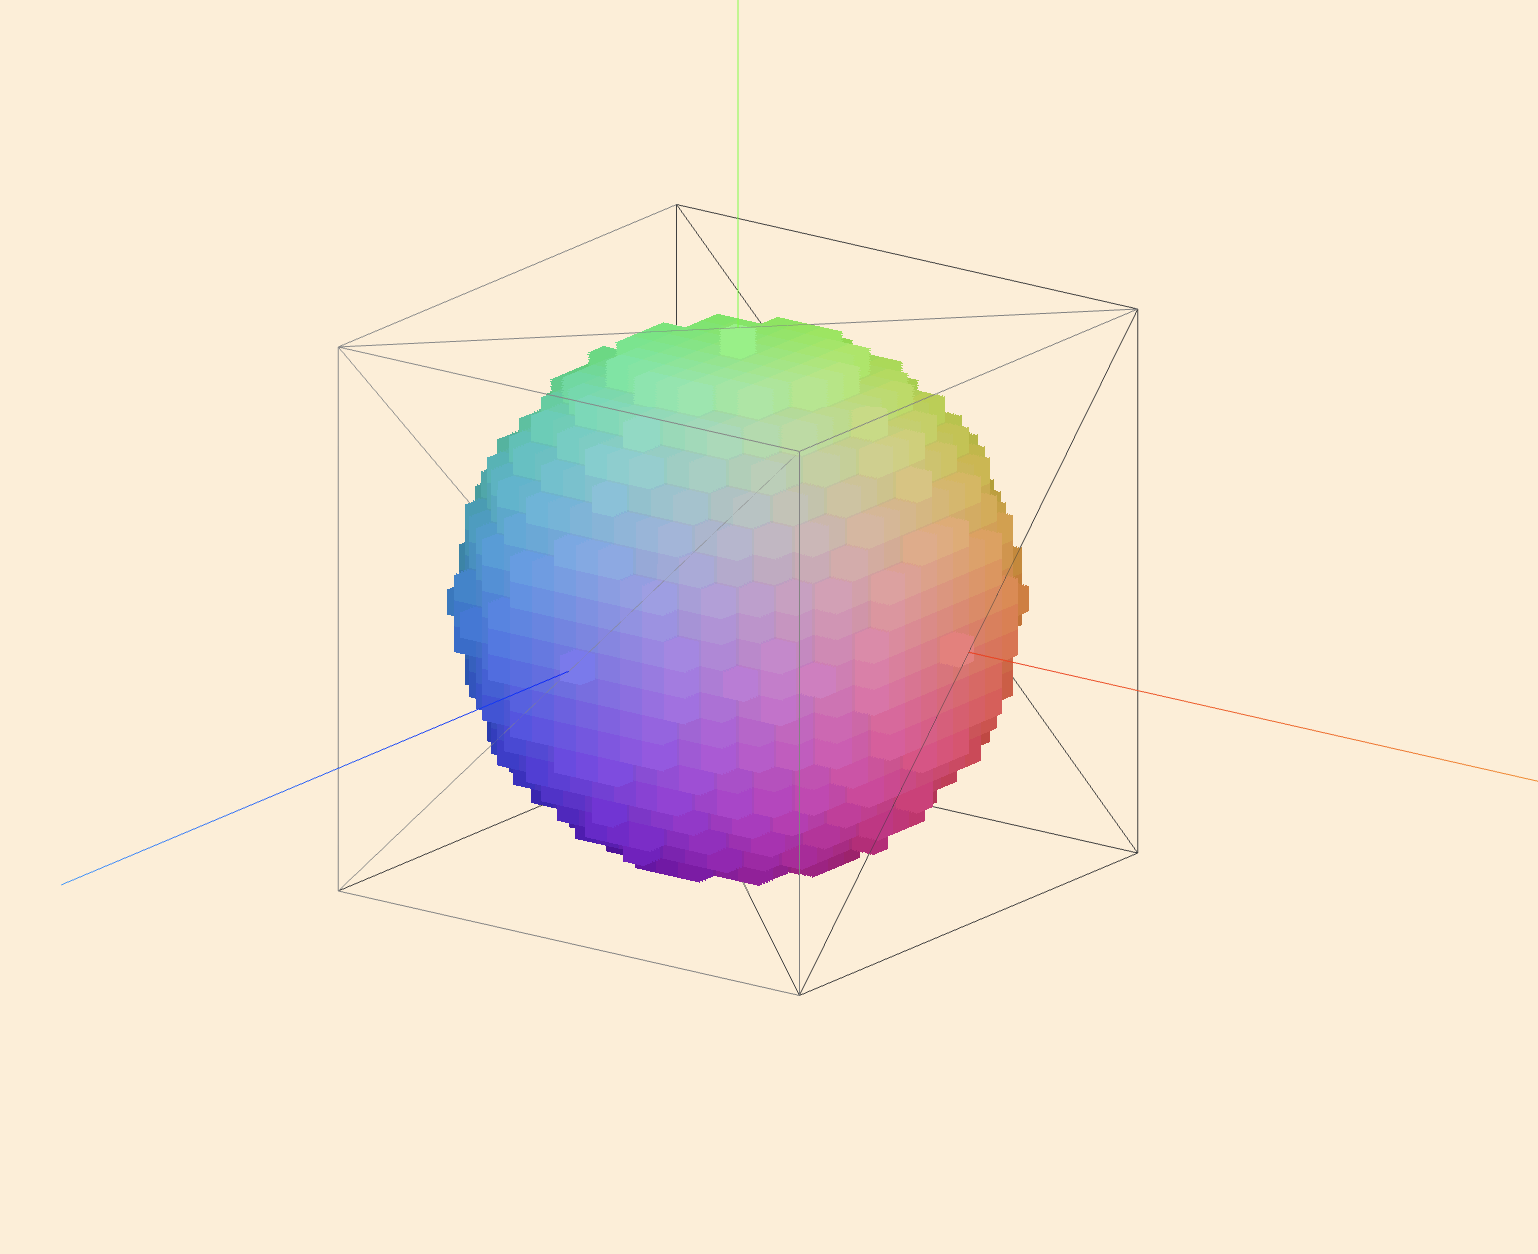
\includegraphics[width=0.7\textwidth]{position.png}
  \caption{Visualisation rending the voxel volume colouring each voxel by its center position.}
\end{figure}
\FloatBarrier

A significant amount of time was invested in calculating per ``face'' normals so that proper shading could be achieved. The technique used for this was inspired by a forum post \cite{reddit} suggesting taking the maximum component of the direction from the voxel center to the hit position. Although, despite this insight and having tried an implementation of this, the result was not successful. This was likely attributed to the inaccuracies of the fixed step size ray marching approach being taken here. An attempt was also made at implementing the \gls{dda} so that correct and accurate hit positions could be obtained, although this implementation was not completed within the project timeline. This can be attributed to difficulties extrapolating existing documented 2D solutions into the 3D case, as well as converting calculations to use vector operations as opposed to calculating axis step components individually. The two primary resources followed when attempting to implement this algorithm were ``Lode's Computer Graphics Tutorial - Raycasting'' \cite{dda:article} and ``An Overview of the Fast Voxel Traversal Algorithm'' \cite{dda:github}; both of which are exceptionally well-written resources.

\subsection{Performance}

In terms of the measured performance of the solution, the renders seen above where created using the following key settings, maxSteps: 100, stepSize: 0.01, resolution (voxel): 21, resolution (display): 1080p. These settings are the key factors that change the renders performance. Given my systems configuration with an M1 Pro processor and 32GB of \gls{ram} I was able to render these visualisations interactively in the browser at a locked 120 \gls{fps} (the maximum refresh rate supported by the laptops in-built display).

\subsection{Risk Management}
Thankfully, being a software application, there is a negligible chance of physical risks associated with this project. Despite this, there are still some minimal data-related risks present which have been accounted for as follows. Data stored in a single place can be susceptible to loss from hardware failure or by misplacing the physical device. To combat this, Git version control has been used to both keep track of incremental program changes on a line-by-line basis, as well as keep a cloud-based backup through the GitHub service \cite{github}. Another crucial aspect that must be considered when working on a programming project is the data involved and the security and privacy expected when handling it. In the case of this voxel engine, there is no sensitive currently being handled.

\subsection{Ethical Considerations}
Ethics are an important consideration when completing any project. For Engineers, we must look to the Engineers Australia Guidelines \cite{ethics} to aid in our professional conduct. Firstly, regarding codes 1.1, 1.3, 3.1, and 3.3, in summary, one must act in good conscience, respect dignity, uphold trustworthiness, and honestly communicate. This has been upheld throughout this project via diligent citation and referencing of a vast number of helpful resources, giving credit where credit is due. The codes described competent practising under section 2 which has also been upheld by my continued effort to stay up to date with the constantly evolving field of software and technology. I do this out of passion but also in the interest of always striving to produce a clean, maintainable software solution that follows best practices such as \gls{dry} mentioned previously.

\subsection{Sustainable Development Principles}
Sustainability is another key aspect that must be taken into account when undertaking any engineering project. Being a small software-based project it is fortunate that this project has a very limited impact in terms of environmental sustainability. The one main impact it does have however is the power consumption of the hardware it is run on. In an attempt to minimise this, developers such as myself must strive to write efficient code that effectively uses compute cycles. So far, this has been implemented in this project by utilising the \gls{gpu} for per-pixel parallel computing.

Another crucial factor relating to sustainability when undertaking this project was the maintainability of the code. As any developer would know, when coming back to one of your projects, or picking up another developers project, it can take a significant amount of time to become acquainted with the code base and understand what is going on. This is doubly true if the code was poorly written and documented. Taking note of this, in order to support sustainable development, it was a goal to write clean and sustainable code from the beginning. This means comments within the source code, meaningful commit messages in version control, progress documentation such as this, as well as clean code structure with sensible variable names.

\subsection{Key Stakeholders}
After accounting for the issues we had with our industry partners, there are now fewer stakeholders in this project. Aside from myself and the academic experience this project will impart to me, there are no other third parties that are significantly invested in the outcome of this thesis. My supervisor, Professor Clinton Fookes, would hold a limited amount of stake in this project as its success or failure could potential reflect on his supervisory presence. Although his support so far through this project's late changes has been warmly welcomed. Since is has ultimately changed to be a student-led project, I suspect his and the investment of \gls{qut} will ultimately be limited.

\section{Conclusion}

Having only a single computer, I cannot attest to performance on other devices, although given that this render performs at double the useful interactive target \gls{fps} of 60, it would not be unreasonable to say that a computer with half the processing power would still be able to render this scene at an interactive rate around the 60 \gls{fps} mark. Especially once taking into consideration the performance improvements that could be achieved by implementation of the more efficient \gls{dda} algorithm. This, coupled with the coming finalisation of the more efficient WebGPU specification and support of this new standard by ThreeJS, paves the way for many future performance improvements. To conclude, the aim of this thesis project was to assess the feasibility of creating a real time voxel rendering engine capable of running in the browser. Having achieved twice the real time \gls{fps} target despite using an inefficient algorithm, It can be observed via these results that this is indeed a feasible goal.

\subsection{Future Work}

As mentioned numerous times throughout this literary piece, there are a number of future improvements that can be made to this work. Firstly and undoubtedly most beneficially would be the implementation of the \gls{dda} algorithm to allow for faster and more accurate ray casting when compared to the fixed step size approach currently implemented. Following on from this, as a by product of the the \gls{dda} algorithm, per ``face'' normal vectors will be know for each voxel allowing for stylised voxel shading as opposed to the position or depth based shading present currently. Lastly, with the potential to turn this project into a completed solution, a more robust voxel data format would need to be implemented. Thus would likely still be a custom format format internally but would include the implementation of file loaders for common formats such as that used for MagicaVoxel \cite{magicavoxel}. This would allow for the import of existing voxel models into the engine such as game assets, medical scans, or any other content in the supported format.

\appendix

\section{Project Timeline}

The table included below outlines all deliverables that where completed as part of this project as well as the presentation still remaining. It also specifies their dependencies along with the expected completion date. A number of these items are outlined by QUT as part of completing an honours thesis in engineering, helping provide good structure to the research. With regards to the interim milestones, these have been goals that I have set myself with the help of communication with the project coordinator, Professor Clinton Fookes and have helped keep the project on track; guiding the production of a working implementation upon completion of this unit.

\begin{center}
  \begin{tabular}{|c|c|c|c|c|c|}
    \hline
    Number & Name                    & Due             & Dependency & Type     & Status     \\
    \hline
    1      & Project Proposal        & W07 Sem 2, 2022 & N/A        & Assessed & Completed  \\
    2      & Get shader working      & W10 Sem 2, 2022 & 1          & Interim  & Completed  \\
    3      & Implement ray marching  & W11 Sem 2, 2022 & 2          & Interim  & Completed  \\
    4      & Render volume to cube   & W12 Sem 2, 2022 & 3          & Interim  & Completed  \\
    5      & Progress Report         & W13 Sem 2, 2022 & 4          & Assessed & Completed  \\
    6      & Oral Presentation       & W03 Sem 1, 2022 & 5          & Assessed & Completed  \\
    7      & Generate voxel sphere   & W08 Sem 1, 2023 & 6          & Interim  & Completed  \\
    8      & Implement ray marching  & W10 Sem 1, 2023 & 7          & Interim  & Completed  \\
    9      & Produce shaded render   & W12 Sem 1, 2023 & 8          & Interim  & Completed  \\
    10     & Final Project Report    & W13 Sem 1, 2023 & 9          & Assessed & Completed  \\
    11     & Final Oral Presentation & End Sem 1, 2023 & 10         & Assessed & Incomplete \\
    \hline
  \end{tabular}
\end{center}

\bibliography{references}

\end{document}
